\documentclass[unicode,12pt]{beamer}
\usepackage{luatexja}
\usepackage[hiragino-pro]{luatexja-preset}
\usepackage{luatexja-fontspec}
\renewcommand{\kanjifamilydefault}{\gtdefault}

\setmonofont{x14y24pxHeadUpDaisy}
\newfontfamily{\magnolia}{Magnolia Script}
\newfontfamily{\brush}{Brush Script MT}

\usepackage{luatexja-ruby}
\usepackage{url}
\usepackage{listings}

\lstdefinelanguage{dhall}{
  keywords={let, in},
  keywordstyle=\color{main}\bfseries,
  keywords=[2]{Bool, Integer, Double, Text, List, Optional},
  keywordstyle=[2]\color{accent}\bfseries,
  identifierstyle=\color{text},
  sensitive=false,
  comment=[l]{--},
  %morecomment=[s]{{-}{-}},
  commentstyle=\color{subtext}\ttfamily,
  stringstyle=\color{main}\ttfamily,
  morestring=[b]',
  morestring=[b]"
}

\lstdefinelanguage{yaml}{
  keywords={let, in},
  keywordstyle=\color{main}\bfseries,
  identifierstyle=\color{text},
  sensitive=false,
  comment=[l]{--},
  %morecomment=[s]{{-}{-}},
  commentstyle=\color{subtext}\ttfamily,
  stringstyle=\color{main}\ttfamily,
  morestring=[b]',
  morestring=[b]"
}

\lstset{
   language=dhall,
   extendedchars=true,
   basicstyle=\footnotesize\ttfamily,
   showstringspaces=false,
   showspaces=false,
   tabsize=2,
   breaklines=true,
   showtabs=false
}

\definecolor{main}{RGB}{49,118,137}
\definecolor{accent}{RGB}{220,94,74}
\definecolor{text}{RGB}{50,50,50}
\definecolor{subtext}{RGB}{80,80,80}

\usetheme{Copenhagen}
\usecolortheme{beaver}
\setbeamertemplate{footline}[page number]

\setbeamercolor{alerted text}{fg=accent}
\setbeamercolor{background canvas}{bg=white}
\setbeamercolor{block body alerted}{bg=normal text.bg!90!black}
\setbeamercolor{block body}{bg=normal text.bg!90!black}
\setbeamercolor{block body example}{bg=normal text.bg!90!black}
\setbeamercolor{block title alerted}{use={normal text,alerted text},fg=alerted text.fg!75!normal text.fg,bg=normal text.bg!75!black}
\setbeamercolor{block title}{bg=main}
\setbeamercolor{block title example}{use={normal text,example text},fg=example text.fg!75!normal text.fg,bg=normal text.bg!75!black}
\setbeamercolor{fine separation line}{}
\setbeamercolor{frametitle}{fg=main}
\setbeamercolor{item projected}{fg=subtext}
\setbeamercolor{normal text}{fg=subtext}
\setbeamercolor{palette sidebar primary}{use=normal text,fg=normal text.fg}
\setbeamercolor{palette sidebar quaternary}{use=structure,fg=structure.fg}
\setbeamercolor{palette sidebar secondary}{use=structure,fg=structure.fg}
\setbeamercolor{palette sidebar tertiary}{use=normal text,fg=normal text.fg}
\setbeamercolor{section in sidebar}{fg=brown}
\setbeamercolor{section in sidebar shaded}{fg=grey}
\setbeamercolor{separation line}{}
\setbeamercolor{sidebar}{bg=red}
\setbeamercolor{sidebar}{parent=palette primary}
\setbeamercolor{structure}{bg=white, fg=main}
\setbeamercolor{subsection in sidebar}{fg=brown}
\setbeamercolor{subsection in sidebar shaded}{fg=grey}
\setbeamercolor{title}{fg=main}
\setbeamercolor{titlelike}{fg=main}

\newlength{\mytotalwidth}
\mytotalwidth=\dimexpr\linewidth-5mm
\newlength{\mycolumnwidth}
\mycolumnwidth=\dimexpr\mytotalwidth-5mm

\renewcommand*{\thefootnote}{\fnsymbol{footnote}}

\renewcommand{\UrlFont}{\ttfamily\scriptsize}

\title{並列並行言語Haskell}
\author[@syocy]{
    \frame{
\includegraphics[width=1cm]{icon.jpg}}\\%
    \vspace{0.5em}%
    @syocy%
}

%\institute{Engineering team}
\date{2018-11-10}

\begin{document}

\begin{frame}[plain]\frametitle{}
  \titlepage
\end{frame}

\section{}

\begin{frame}[plain]{参考書}
  \begin{columns}[totalwidth=\mytotalwidth]
    \begin{column}[T]{0.5\mycolumnwidth}
      \centering
      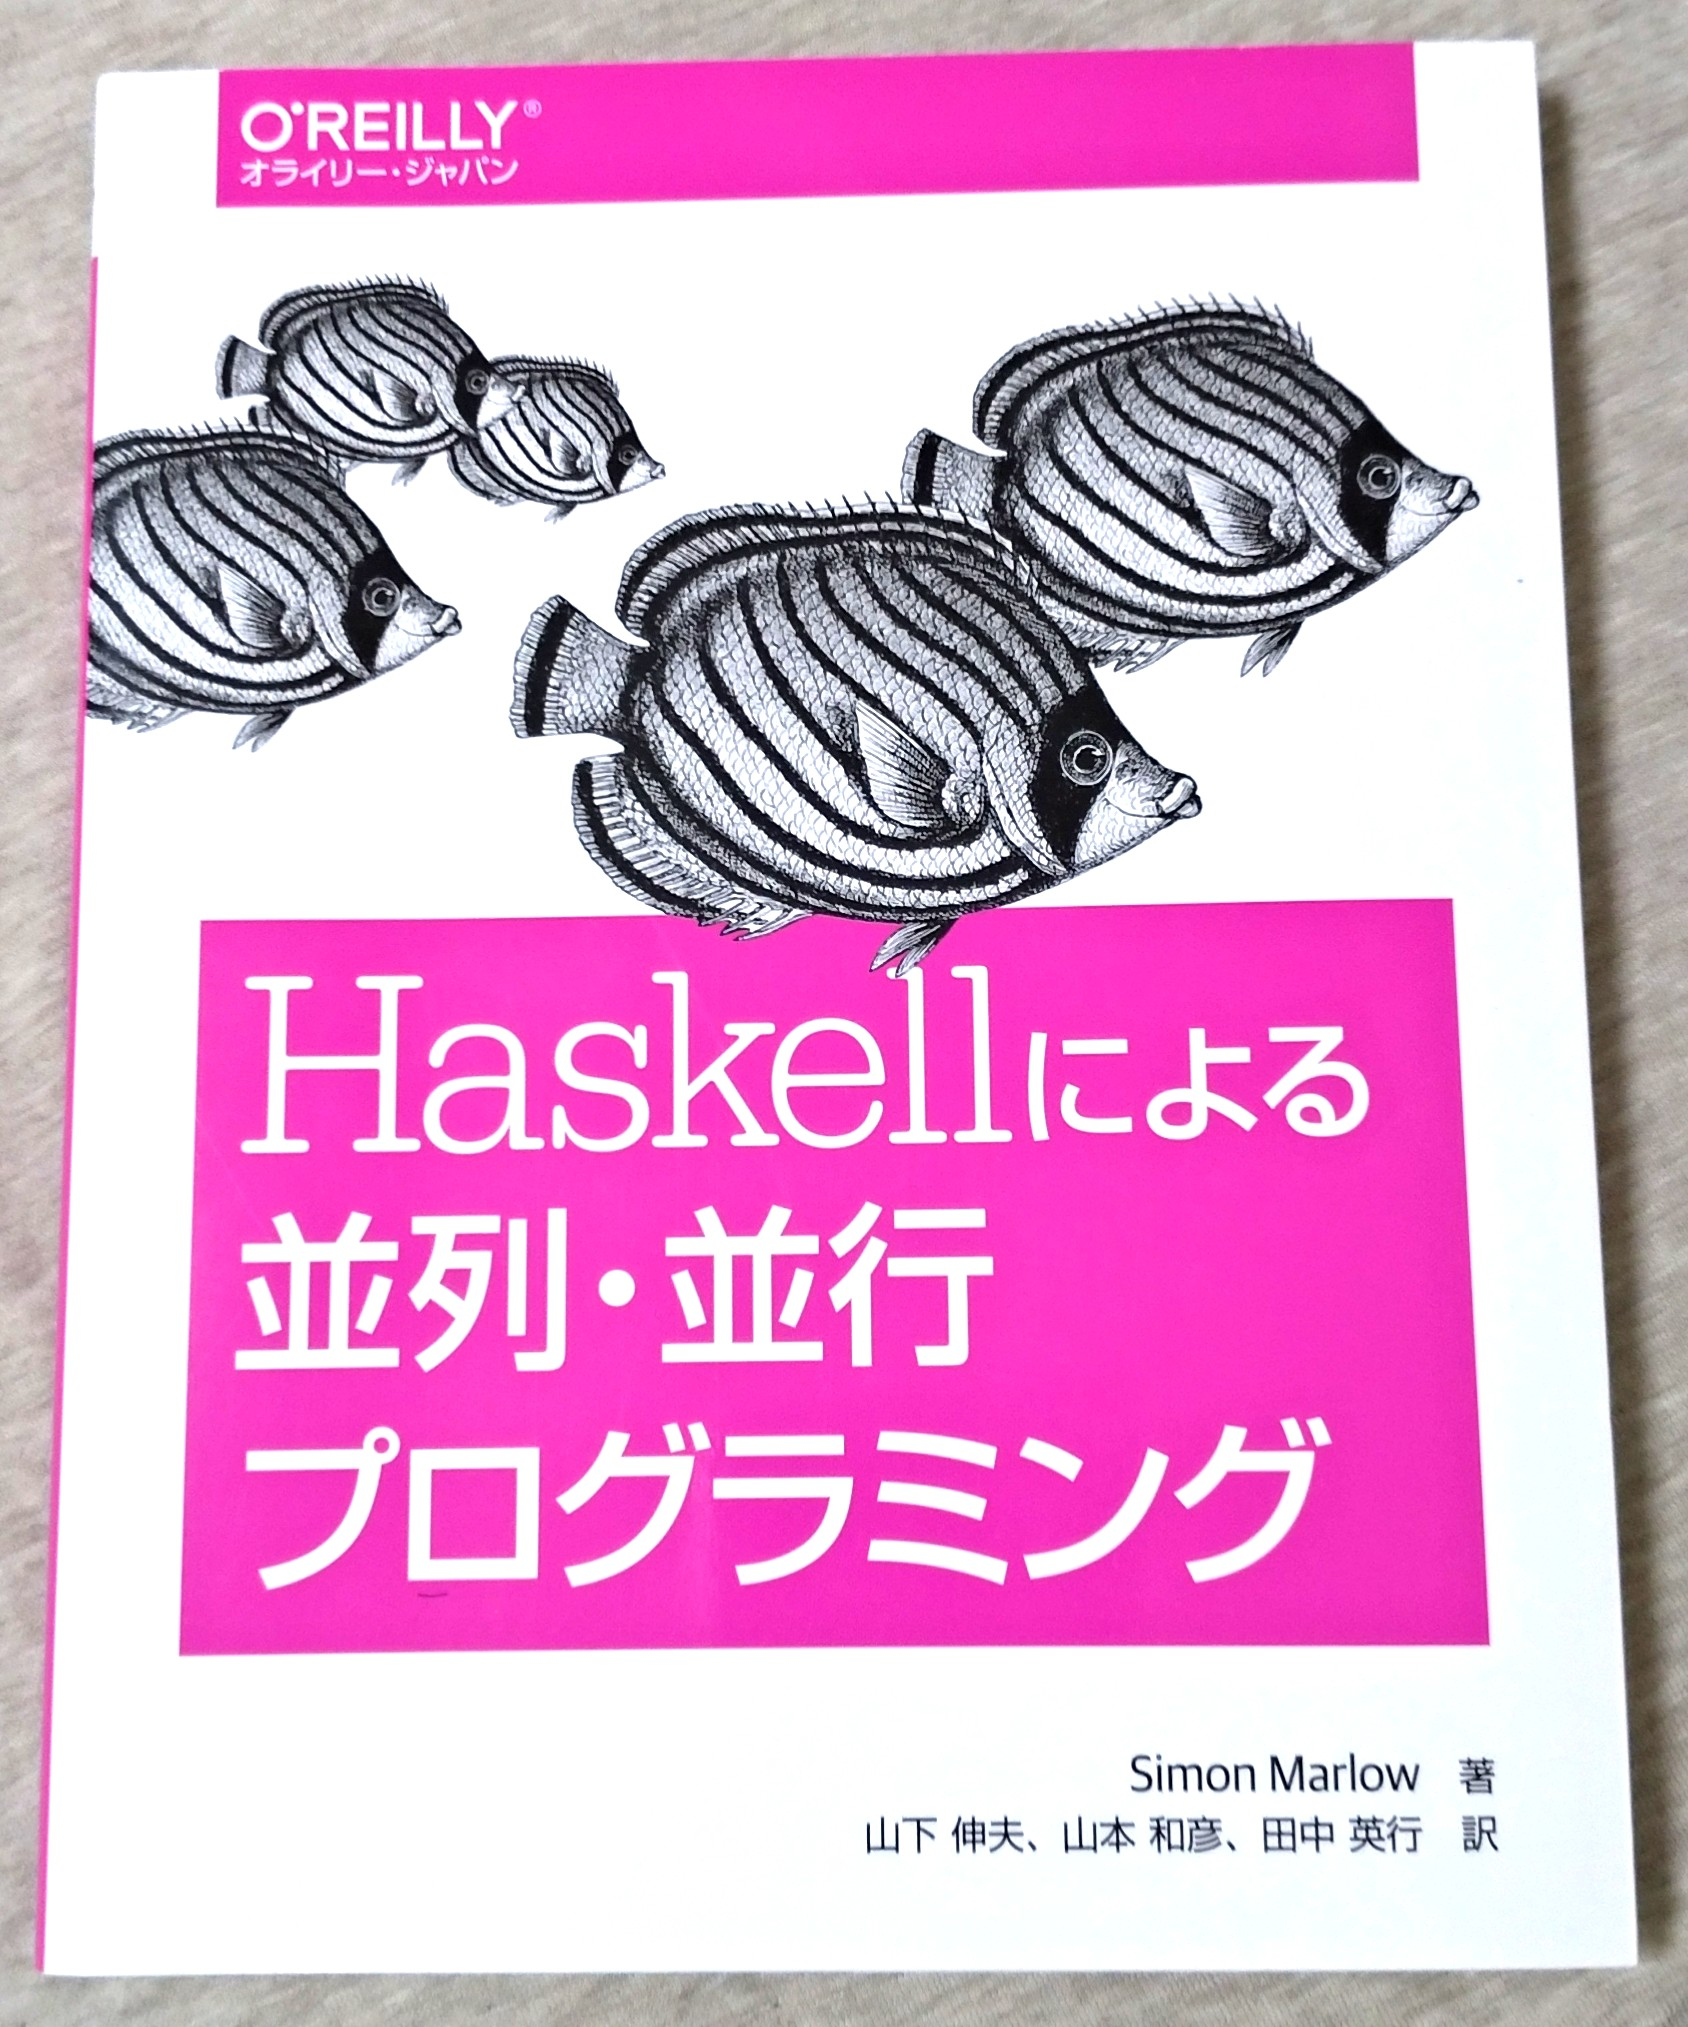
\includegraphics[width=\columnwidth]{pic/book.jpg} \\
      Haskellによる並列・並行\\ プログラミング
    \end{column}
    \begin{column}[t]{0.5\mycolumnwidth}
      \begin{itemize}
      \item GHCの主要開発者 Simon Marlow 自身による並列・並行 Haskell の解説書
      \item 並列・並行の様々なアイデアが紹介されており Haskell ユーザ以外にもおすすめ
      \end{itemize}
    \end{column}
  \end{columns}
  \centering
\end{frame}

\section{並列・並行をやるモチベーション}

\begin{frame}{プロセッサ性能トレンド}
  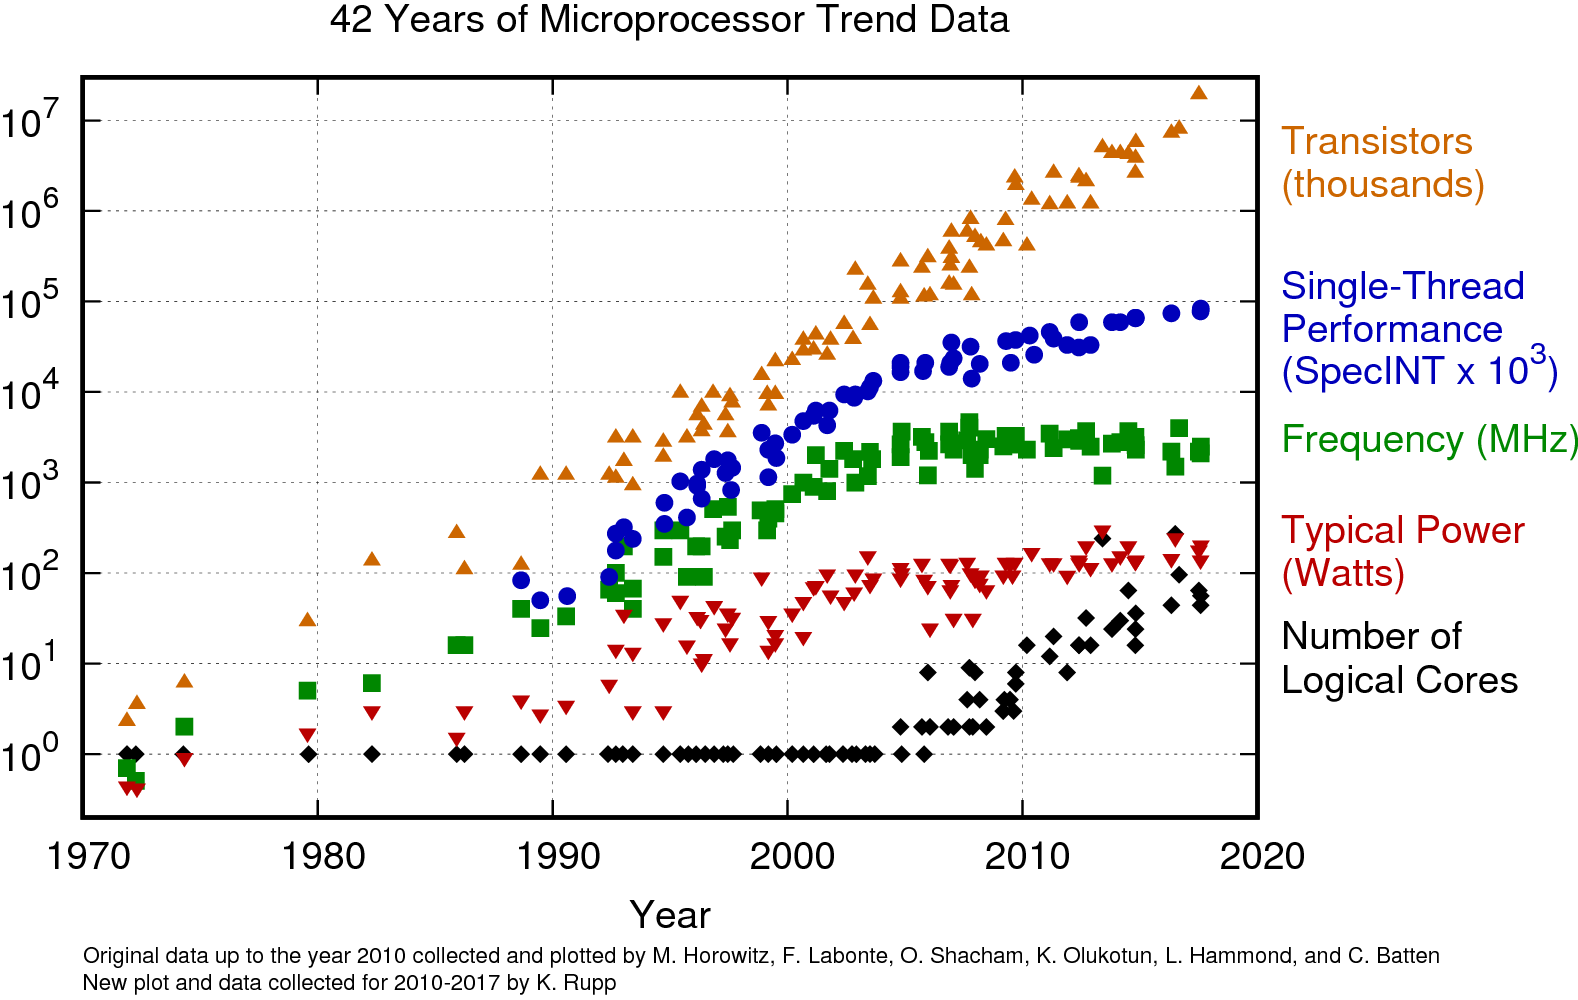
\includegraphics[width=\textwidth]{pic/42-years-processor-trend.png}
\end{frame}

\begin{frame}{プロセッサ性能トレンド}
  \begin{columns}[totalwidth=\mytotalwidth]
    \begin{column}[T]{0.3\mycolumnwidth}
      \centering
      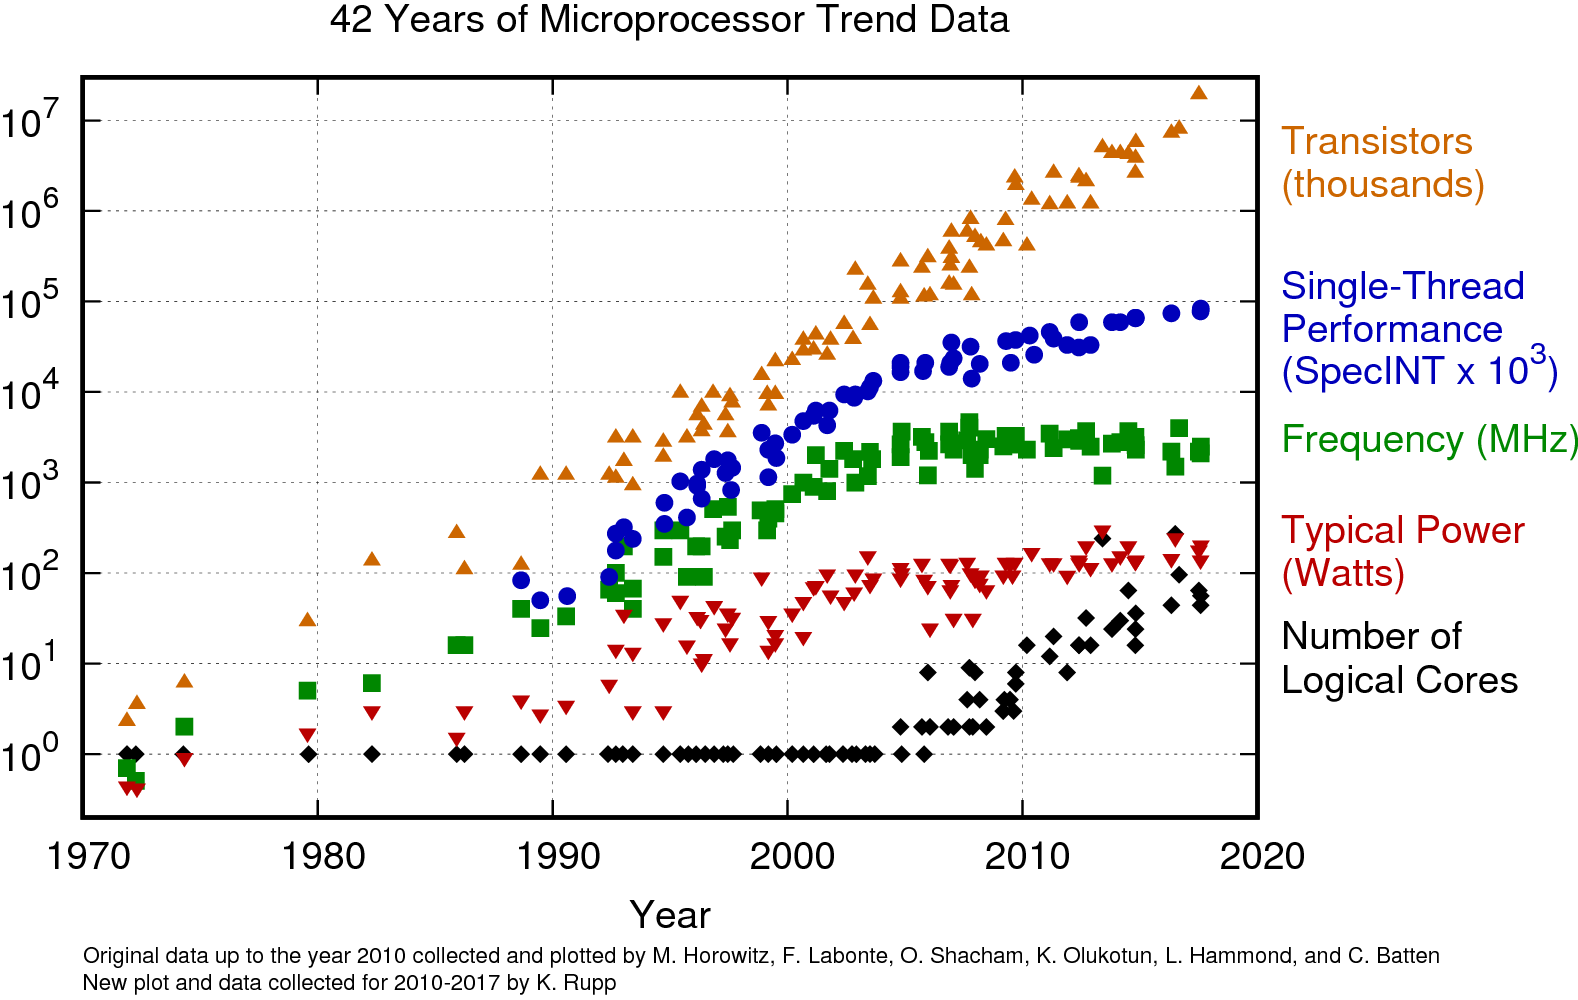
\includegraphics[width=\columnwidth]{pic/42-years-processor-trend.png}
    \end{column}
    \begin{column}[t]{0.7\mycolumnwidth}
      \begin{itemize}
      \item シングルスレッド性能は伸び悩んできている
      \item 一方で論理コア数は順調に増えてきている
      \item \alert{現代のプロセッサの能力を引き出すにはコア数を活かすプログラミングが必要}
      \end{itemize}
    \end{column}
  \end{columns}
\end{frame}

\begin{frame}{お求めやすくなったメニーコアCPU}
  \begin{itemize}
  \item 10以上\footnote{メニーコアの定義は曖昧。ここでは物理10コア以上をメニーコアと呼ぶことにする。}
    の物理コアを持つCPUがご家庭でも手に入れられるお値段になった
    \end{itemize}
  \begin{tabular}{llll} \hline
    CPU & Core & Freq & Price \\ \hline
    Ryzen TR 2990WX & 32-core 64-thread & 3.0GHz & \$1799 \\
    Ryzen TR 2950X & 16-core 32-thread & 3.5GHz & \$899 \\
    Ryzen TR 1920X & 12-core 24-thread & 3.5GHz & \$399 \\
    \hline
  \end{tabular}
\end{frame}

\begin{frame}{並列並行言語の台頭}
  最近話題の言語はコアな部分に並列並行機能を備えていることが多い \\
  → 並列並行の重要性が意識され始めた
  \begin{itemize}
  \item Go: goroutine(コルーチン)を持つ
  \item Erlang, Elixir: VMが軽量プロセスを持つ
  \item Rust: メモリー安全性が並行性にも及ぶことを強調している
  \end{itemize}
  Haskell はどうか?
\end{frame}

\section{並列・並行とHaskell}

\begin{frame}{並列・並行とHaskell}
  Haskell (GHC) は古くから並列・並行を考えて設計されてきた
  \begin{itemize}
  \item 1997年にライブラリではなく実行時システムとして並行性をサポートすることが決定
  \item 2004年に実行時システムを共有メモリのマルチプロセッサ上で並列に動作させることが決定
  \item 2009年の論文 ``Runtime support for multicore Haskell''
  \end{itemize}
\end{frame}

\begin{frame}{並列・並行のためのよい性質}
  Haskell は並列・並行のためのよい特徴を持つ
  \begin{itemize}
  \item Haskell は純粋なコードと副作用(IOなど)を含むコードを分離できる
    \begin{itemize}
    \item 並列性は\alert{決定的}: 並列度や実行環境が変わろうと結果は変わらない
    \end{itemize}
  \item 実行時システムが\alert{軽量スレッド}をサポートする
    \begin{itemize}
    \item よく並行性の実現にはスレッドが用いられるが、
    \item あたかも普通の(OS)スレッドのように使えるものが、普通のスレッドよりはるかに軽く動作する
    \end{itemize}
  \end{itemize}
  Haskell 使うっきゃない!
\end{frame}

\section{並列・並行(・分散)の意味}

\begin{frame}{並列・並行(・分散)って?}
  これまで断りなく使ってきた言葉
  \begin{itemize}
  \item 並列(parallel)
  \item 並行(concurrent)
  \item (分散(distributed))
  \end{itemize}
  に違いはあるの?
\end{frame}

\begin{frame}{並列と並行}
  \begin{itemize}
  \item 並列(parallel): 同時に走らせることで処理を\alert{高速化}したい
    \begin{itemize}
    \item 用例: n並列、並列ダウンロード、GPU並列計算
    \end{itemize}
  \item 並行(concurrent): \alert{そもそも}同時にしたい処理がある
  \end{itemize}
\end{frame}

\begin{frame}{分散}
  分散は並列・並行とは異なる特徴を持つ
  \begin{itemize}
  \item 分散(distributed): 複数のマシンを使う処理のこと
    \begin{itemize}
    \item 通信時間がかかるため、基本共有メモリを持たない
    \item 一部のマシンがダウンするかもしれない
    \item マシンによって性質が異なることがありうる
    \end{itemize}
  \end{itemize}
  このスライドでは分散にはあまり触れない
\end{frame}

\section{並列・並行のコード}

\begin{frame}{並列・並行のコード}
  \begin{itemize}
  \item 並列 Haskell は Haskell 特有の性質を理解していないと把握しづらい
  \item そのためまずは並行 Haskell (軽量スレッド) から見ていく
  \end{itemize}
\end{frame}

\subsection{軽量スレッドを明示的に使う}

\begin{frame}{軽量スレッドを作成する}
  \lstinputlisting[breaklines=false,numbers=left,language=haskell,firstline=40,lastline=49]{../src/Lib.hs}
\end{frame}

\begin{frame}{軽量スレッドを作成する}
  \begin{itemize}
  \item \alert{\ttfamily{async}} 関数で軽量スレッドを作る
    \begin{itemize}
    \item async パッケージに入っている
    \item 実体は標準関数 \ttfamily{forkIO} の薄いラッパー。
      \ttfamily{async} の方がより安全で便利なので利用推奨。
    \end{itemize}
    \item \ttfamily{wait} 関数で軽量スレッドの終了を待つこともできる
  \end{itemize}
\end{frame}

\begin{frame}{スレッド間通信}
  STMでアトミックなMapを作る例
  \lstinputlisting[breaklines=false,numbers=left,language=haskell,firstline=60,lastline=72]{../src/Lib.hs}
\end{frame}

\begin{frame}{スレッド間通信}
  スレッド間通信には大まかに2つの方法がある
  \begin{itemize}
  \item {\ttfamily MVar}
    \begin{itemize}
    \item シンプルな同期変数
    \item アクセスの\alert{公平性}が保証される
    \item MVarによるチャネルとセマフォの実装がある
    \end{itemize}
  \item STM(Software Transactional Memory)
    \begin{itemize}
    \item 共有状態の読み書きに\alert{トランザクション}の概念を導入
      \begin{itemize}
      \item 割り込まれない一連の読み書きブロック
      \item 途中で失敗したらなかったことにしてリトライできる
      \end{itemize}
    \item STMによるチャネル、キュー、制限付きキュー、セマフォ等の実装がある
    \end{itemize}
  \end{itemize}
\end{frame}

\begin{frame}{宣伝: A Tour of Go in Haskell\footnote{\url{https://a-tour-of-go-in-haskell.syocy.net/ja_JP/index.html}}}
  \centering
  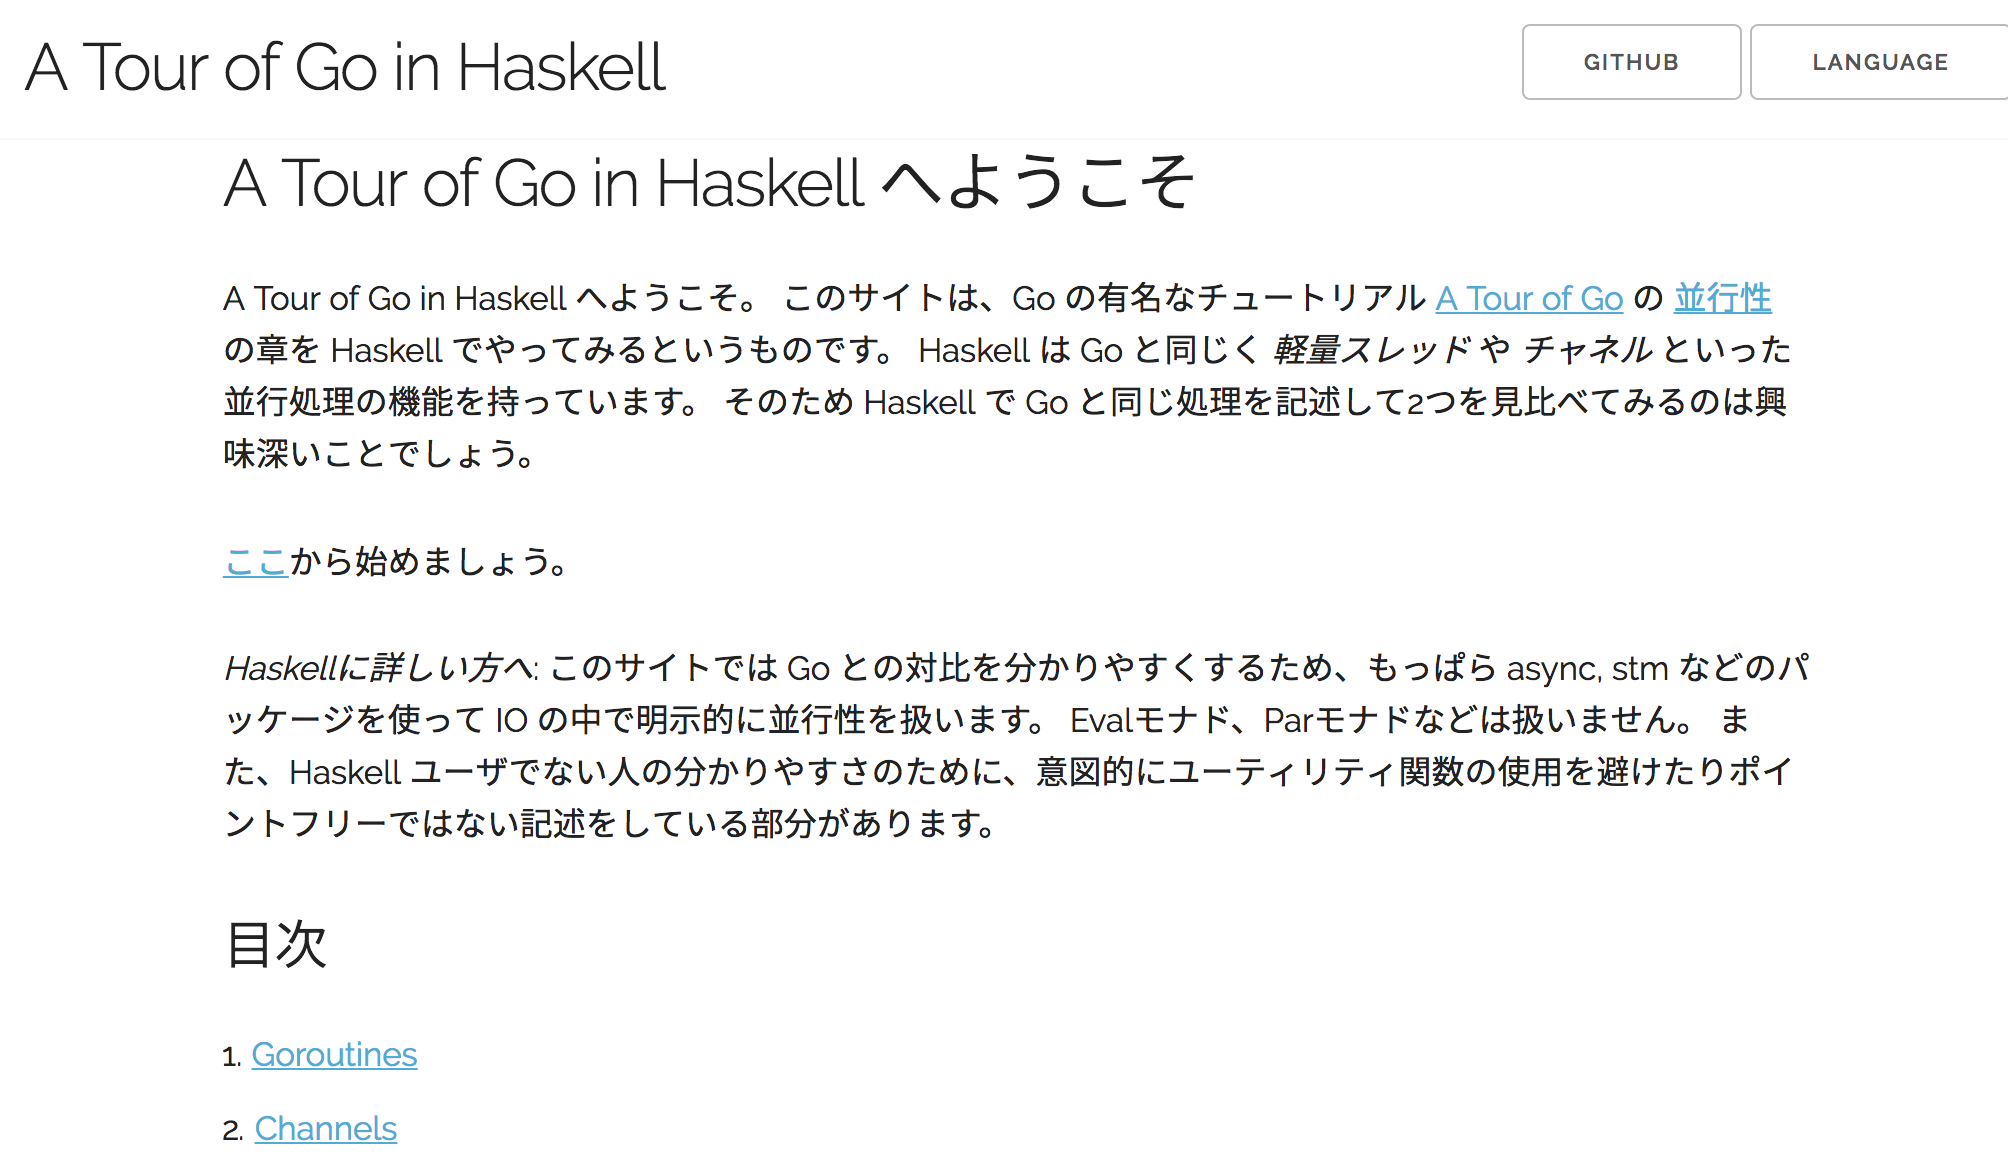
\includegraphics[width=.55\textwidth]{pic/a_tour_of_go_in_haskell.png}
  \begin{itemize}
  \item Go のチュートリアル ``A Tour of Go'' の並行性の章を Haskell で書いた
  \item 並行構文の軽さは Go と Haskell で同じくらい
  \item STMがあるぶん Haskell の方がうまく書ける例も
  \end{itemize}
\end{frame}

\subsection{評価順序を改変する}

\begin{frame}{}

\end{frame}

\section{より高レイヤーのツール}

\begin{frame}{自動的な並列化}
  \begin{itemize}
  \item Parモナド
    \begin{itemize}
    \item データフロー並列: データフローグラフの並列にできるところを並列化
    \item パイプライン並列: データ処理パイプラインの各段を並列化
    \end{itemize}
  \item Haxl
    \begin{itemize}
    \item データソースへのクエリを自動的に並列化する
    \item Facebookのスパムフィルタで使われている
    \end{itemize}
  \end{itemize}
\end{frame}

\begin{frame}{行列計算の並列化}
  \begin{itemize}
  \item repa
    \begin{itemize}
      \item 行列計算について自動並列の一種であるデータ並列を導入する
    \end{itemize}
  \item accelerate
    \begin{itemize}
      \item 行列計算の並列化をサポートする
      \item repaと違い、Haskell以外のコードを生成する; GPU, LLVM IR,..
      \end{itemize}
  \end{itemize}
\end{frame}

\begin{frame}{分散プログラミング}
  \begin{itemize}
  \item distributed-process a.k.a. Cloud Haskell
    \begin{itemize}
    \item Haskellに分散プログラミングを導入するフレームワーク
    \item Erlang, Elixirの軽量プロセスに近い実行モデル
    \item とある暗号通貨の実装に使われているらしい
    \end{itemize}
  \end{itemize}
\end{frame}

\begin{frame}{マルチスレッドプロファイリング}
  \begin{itemize}
  \item ThreadScope
    \begin{itemize}
    \item Haskell の実行時プロファイルを可視化してくれるツール
    \item 各OS向けにバイナリ配布されているので導入しやすい
    \end{itemize}
  \end{itemize}
  \centering
  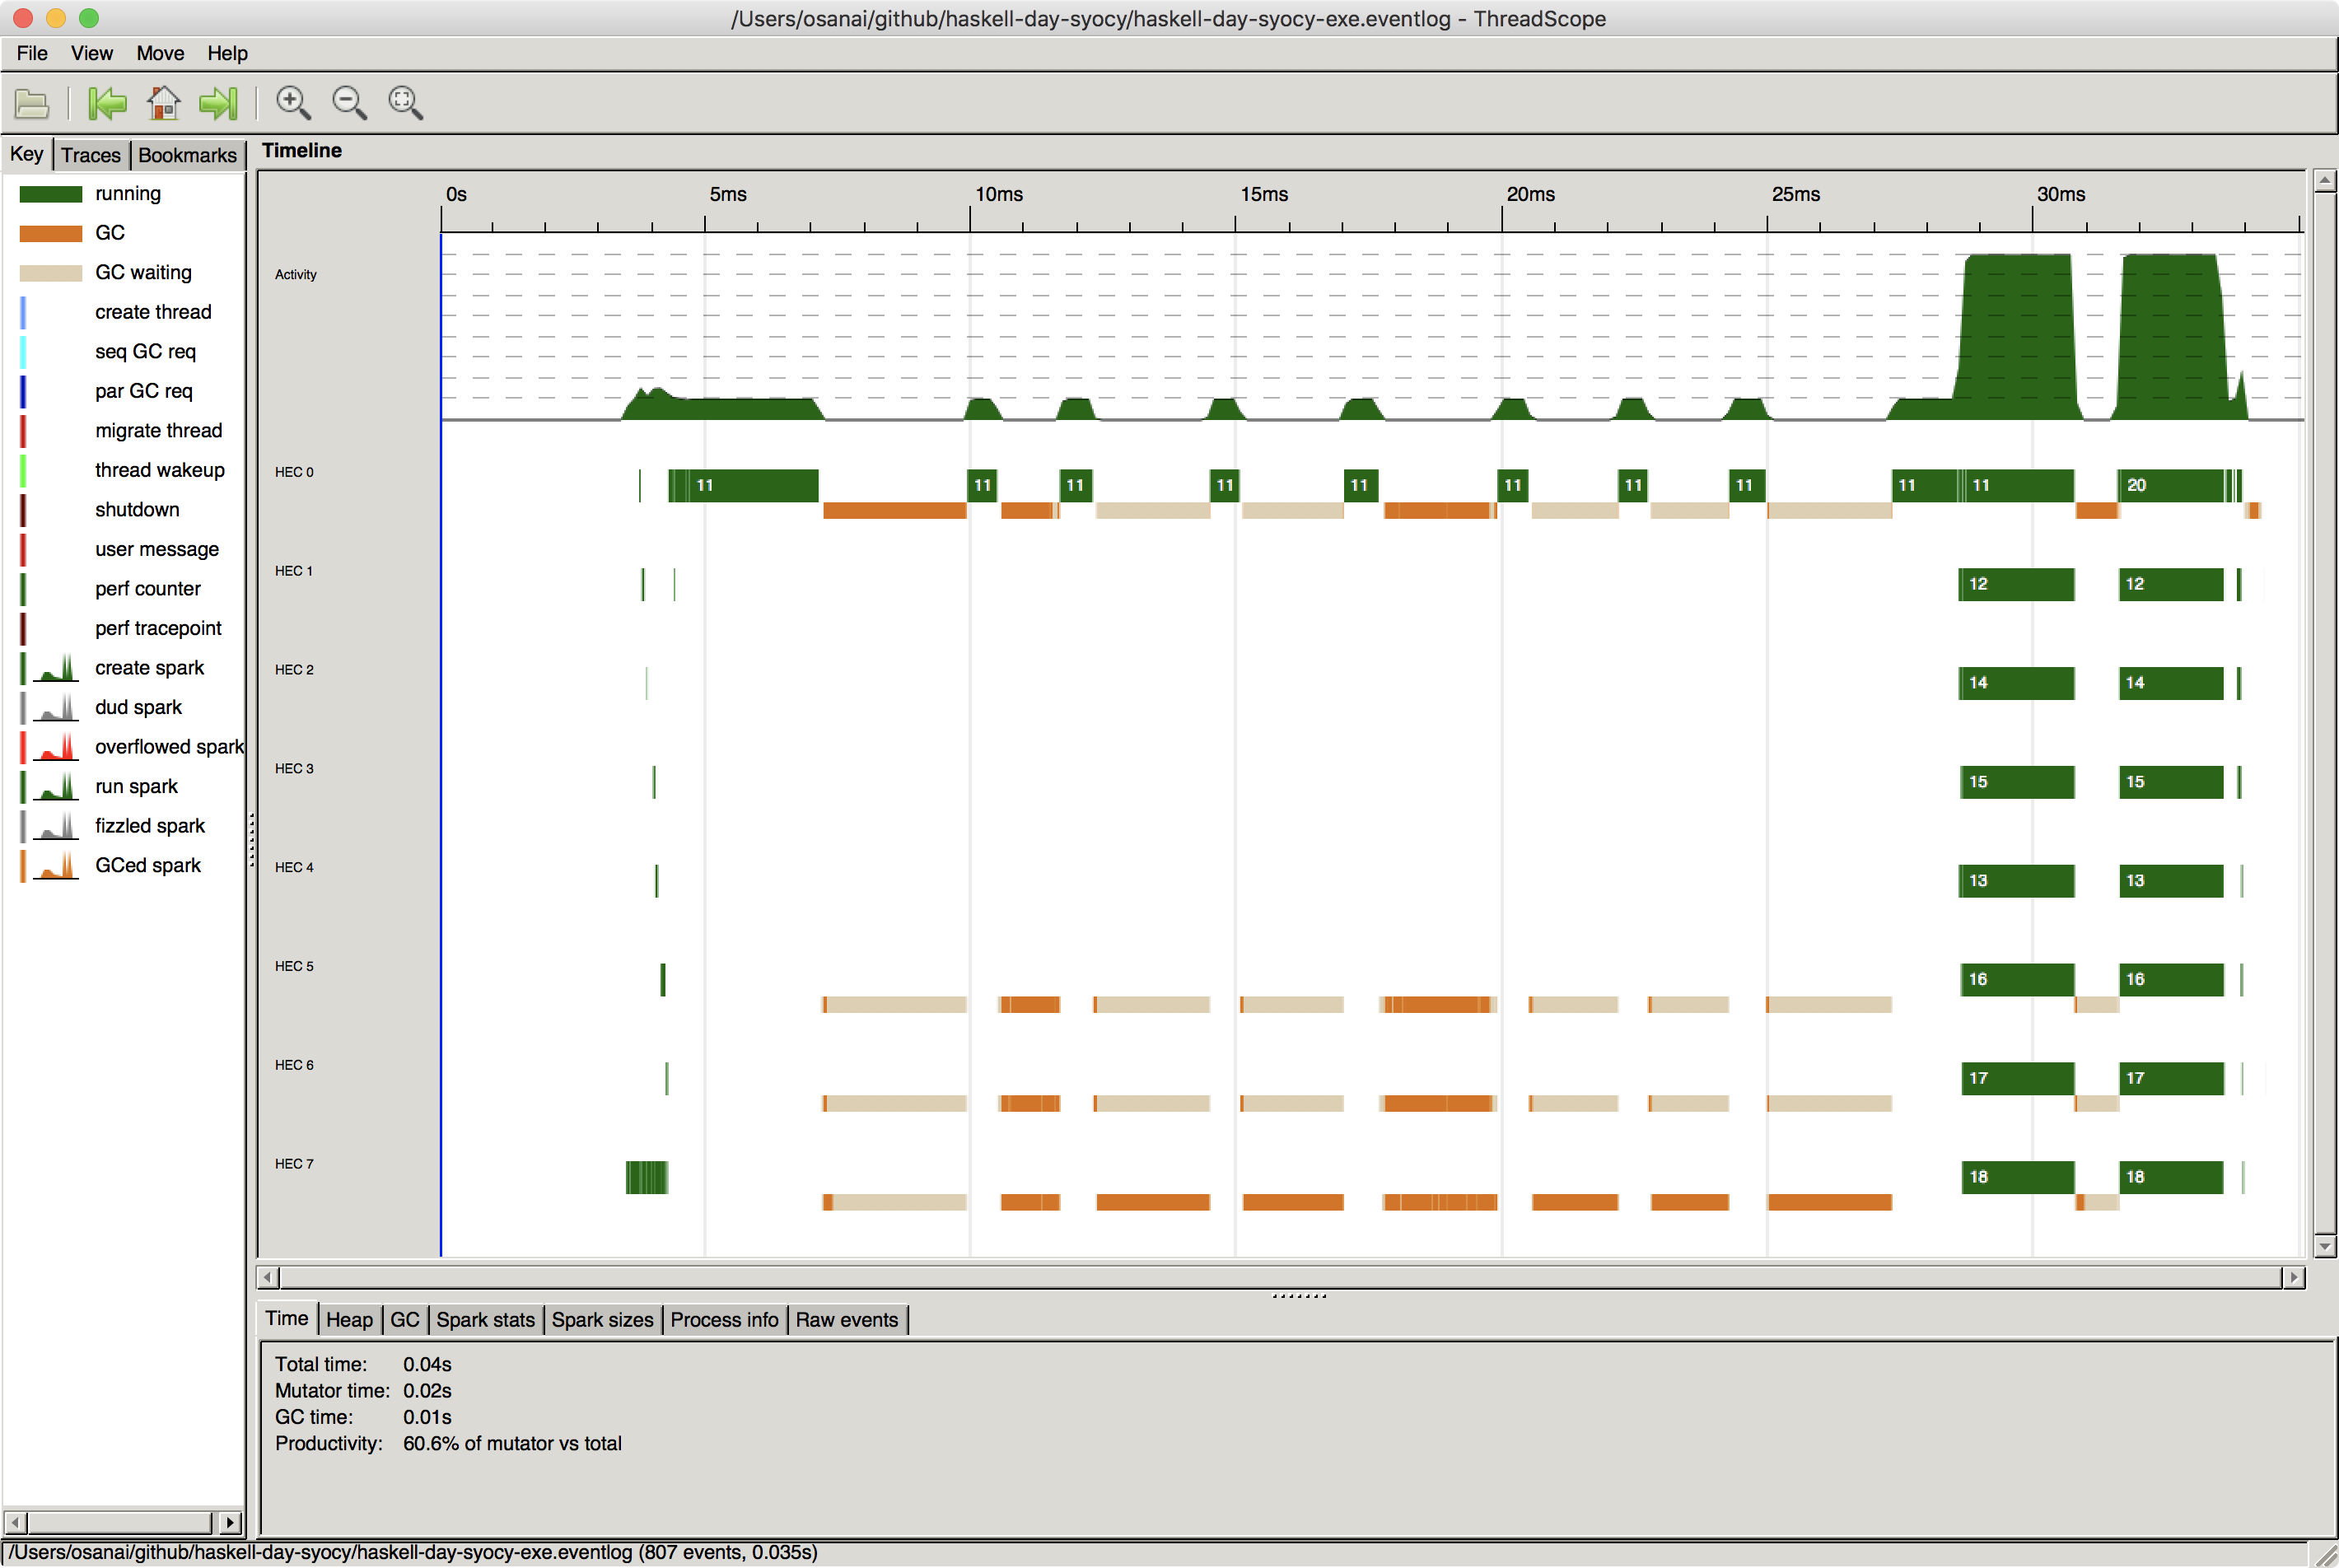
\includegraphics[width=.5\textwidth]{pic/threadscope.png}
\end{frame}

\section{}

\begin{frame}{まとめ}

\end{frame}

\begin{frame}[plain]{補遺: Haskellの並列・並行関連のニュース}
  \begin{enumerate}
  \item ApplicativeDo (GHC 8.0)
  \item Facebook での成果: -qn オプション (GHC 8.2)
  \item GHC の NUMA サポート (GHC 8.2)
  \item 暗号通貨 Cardano は Cloud Haskell を使っている?
  \end{enumerate}
\end{frame}

\begin{frame}[plain]{補遺: 軽量スレッドの消費メモリ(引用)}
  \centering
  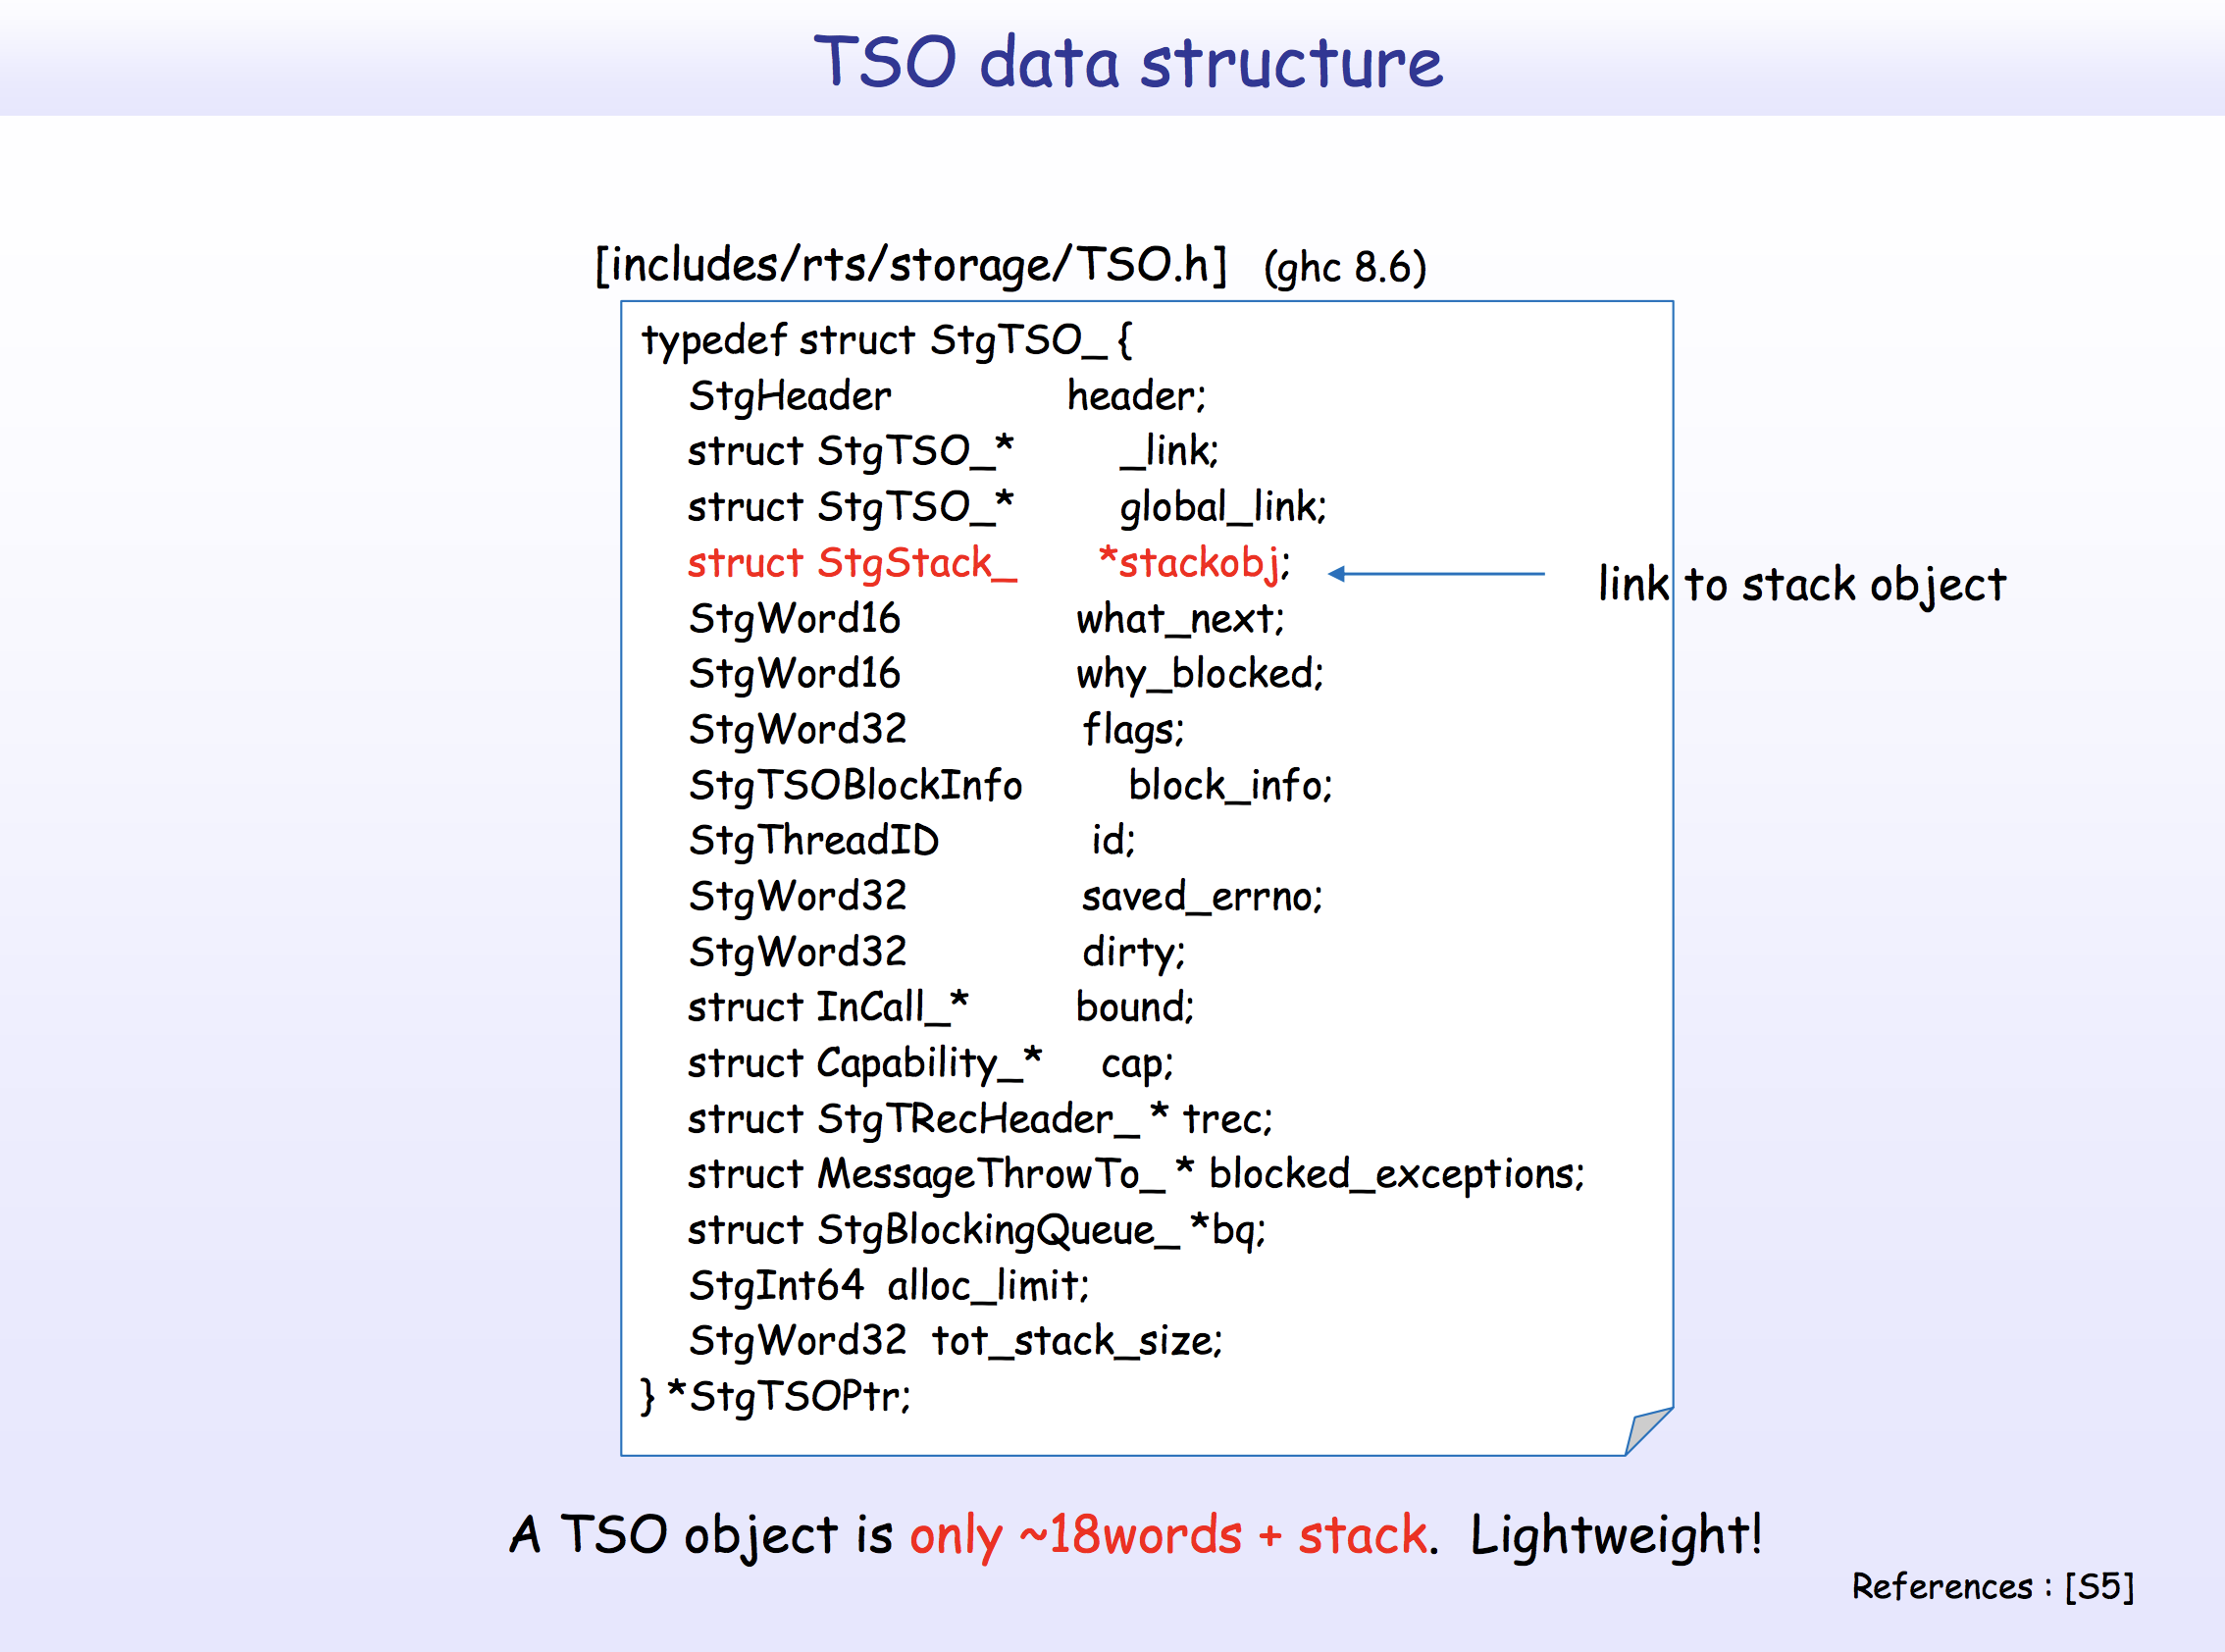
\includegraphics[width=.7\textwidth]{pic/tso.png}
  \footnote{Reference: takenobu-hs, ``haskell-ghc-illustrated'' - \url{https://takenobu-hs.github.io/downloads/haskell_ghc_illustrated.pdf}}
\end{frame}

\end{document}
